\chapter{Implementacija i korisničko sučelje}
		
		
		\section{Korištene tehnologije i alati}
		
\subsection{Komunikacijske platforme}

Tim je ostvarivao komunikaciju putem različitih platformi kako bi osigurao učinkovitu suradnju i komunikaciju među članovima.
Komunikacija unutar tima

\subsubsection{WhatsApp}
WhatsApp poslužio je kao glavna platforma za svakodnevnu komunikaciju unutar 
tima. Ova aplikacija omogućila je brzu razmjenu poruka, datoteka i informacija
, čime je podržala fluidnost timskih interakcija.

\subsubsection{Microsoft Teams}
Microsoft Teams postao je ključna platforma za komunikaciju s profesorima i 
asistentom. Integrirana s drugim alatima iz Microsoft ekosustava, Teams 
omogućava organizaciju sastanaka, dijeljenje dokumenata te olakšava suradnju 
na projektu.

Razvojno okruženje

\subsubsection{IntelliJ IDEA}
IntelliJ IDEA je integrirano razvojno okruženje (IDE) koje pruža napredne 
značajke za Java, Kotlin, Groovy i drugih programskih jezika. Poznat po svojoj 
inteligentnoj podršci za refaktoriranje, automatsko dovršavanje koda te 
integraciji s popularnim alatima poput Mavena i Gradlea.

\subsubsection{Neovim}
Neovim je unaprijeđeni klon klasičnog Vim uređivača teksta. Pruža napredne 
mogućnosti uređivanja teksta, podršku za različite programerske jezike i 
proširivost putem raznih dodataka. Idealno rješenje za korisnike koji cijene 
efikasnost u radu s tekstualnim datotekama.

\subsubsection{Visual Studio Code}
Visual Studio Code je uređivač teksta koji je vrlo brzo postao favorit među
programerima. Danas je gotovo sveprisutan, a svoju popularnost uveliko
duguje moćnoj proširivosti, sa proširenjima za bilo koju potrebu koja se
može zamisliti.

\subsection{Razvoj aplikacije}

Aplikacija je izgrađena koristeći sljedeće tehnologije:

\subsubsection{Backend}

Spring: Framework za Java aplikacije koji omogućuje brz i efikasan razvoj. 
Koristi se za izgradnju robustnih backend komponenti.

\subsubsection{Frontend}

React: Biblioteka za izgradnju korisničkih sučelja u JavaScriptu. Omogućuje 
razvoj visoko modularnih i brzih aplikacija.

JavaScript: Programski jezik koji se koristi u razvoju frontend dijela 
aplikacije.

\subsubsection{Baza podataka}

PostgreSQL: Sustav upravljanja bazama podataka otvorenog koda, sa jakim 
fokusom na ACID principe, i pridržavanje SQL standarda.
			
			
			\eject 
		
	
		\section{Ispitivanje programskog rješenja}
			
			\textbf{\textit{dio 2. revizije}}\\
			
			 \textit{U ovom poglavlju je potrebno opisati provedbu ispitivanja implementiranih funkcionalnosti na razini komponenti i na razini cijelog sustava s prikazom odabranih ispitnih slučajeva. Studenti trebaju ispitati temeljnu funkcionalnost i rubne uvjete.}
	
			
			\subsection{Ispitivanje komponenti}
			\textit{Potrebno je provesti ispitivanje jedinica (engl. unit testing) nad razredima koji implementiraju temeljne funkcionalnosti. Razraditi \textbf{minimalno 6 ispitnih slučajeva} u kojima će se ispitati redovni slučajevi, rubni uvjeti te izazivanje pogreške (engl. exception throwing). Poželjno je stvoriti i ispitni slučaj koji koristi funkcionalnosti koje nisu implementirane. Potrebno je priložiti izvorni kôd svih ispitnih slučajeva te prikaz rezultata izvođenja ispita u razvojnom okruženju (prolaz/pad ispita). }
			
			
			
			\subsection{Ispitivanje sustava}
			
			 \textit{Potrebno je provesti i opisati ispitivanje sustava koristeći radni okvir Selenium\footnote{\url{https://www.seleniumhq.org/}}. Razraditi \textbf{minimalno 4 ispitna slučaja} u kojima će se ispitati redovni slučajevi, rubni uvjeti te poziv funkcionalnosti koja nije implementirana/izaziva pogrešku kako bi se vidjelo na koji način sustav reagira kada nešto nije u potpunosti ostvareno. Ispitni slučaj se treba sastojati od ulaza (npr. korisničko ime i lozinka), očekivanog izlaza ili rezultata, koraka ispitivanja i dobivenog izlaza ili rezultata.\\ }
			 
			 \textit{Izradu ispitnih slučajeva pomoću radnog okvira Selenium moguće je provesti pomoću jednog od sljedeća dva alata:}
			 \begin{itemize}
			 	\item \textit{dodatak za preglednik \textbf{Selenium IDE} - snimanje korisnikovih akcija radi automatskog ponavljanja ispita	}
			 	\item \textit{\textbf{Selenium WebDriver} - podrška za pisanje ispita u jezicima Java, C\#, PHP koristeći posebno programsko sučelje.}
			 \end{itemize}
		 	\textit{Detalji o korištenju alata Selenium bit će prikazani na posebnom predavanju tijekom semestra.}
			
			\eject 
		
		
		\section{Dijagram razmještaja}
			
\begin{figure}[H]
	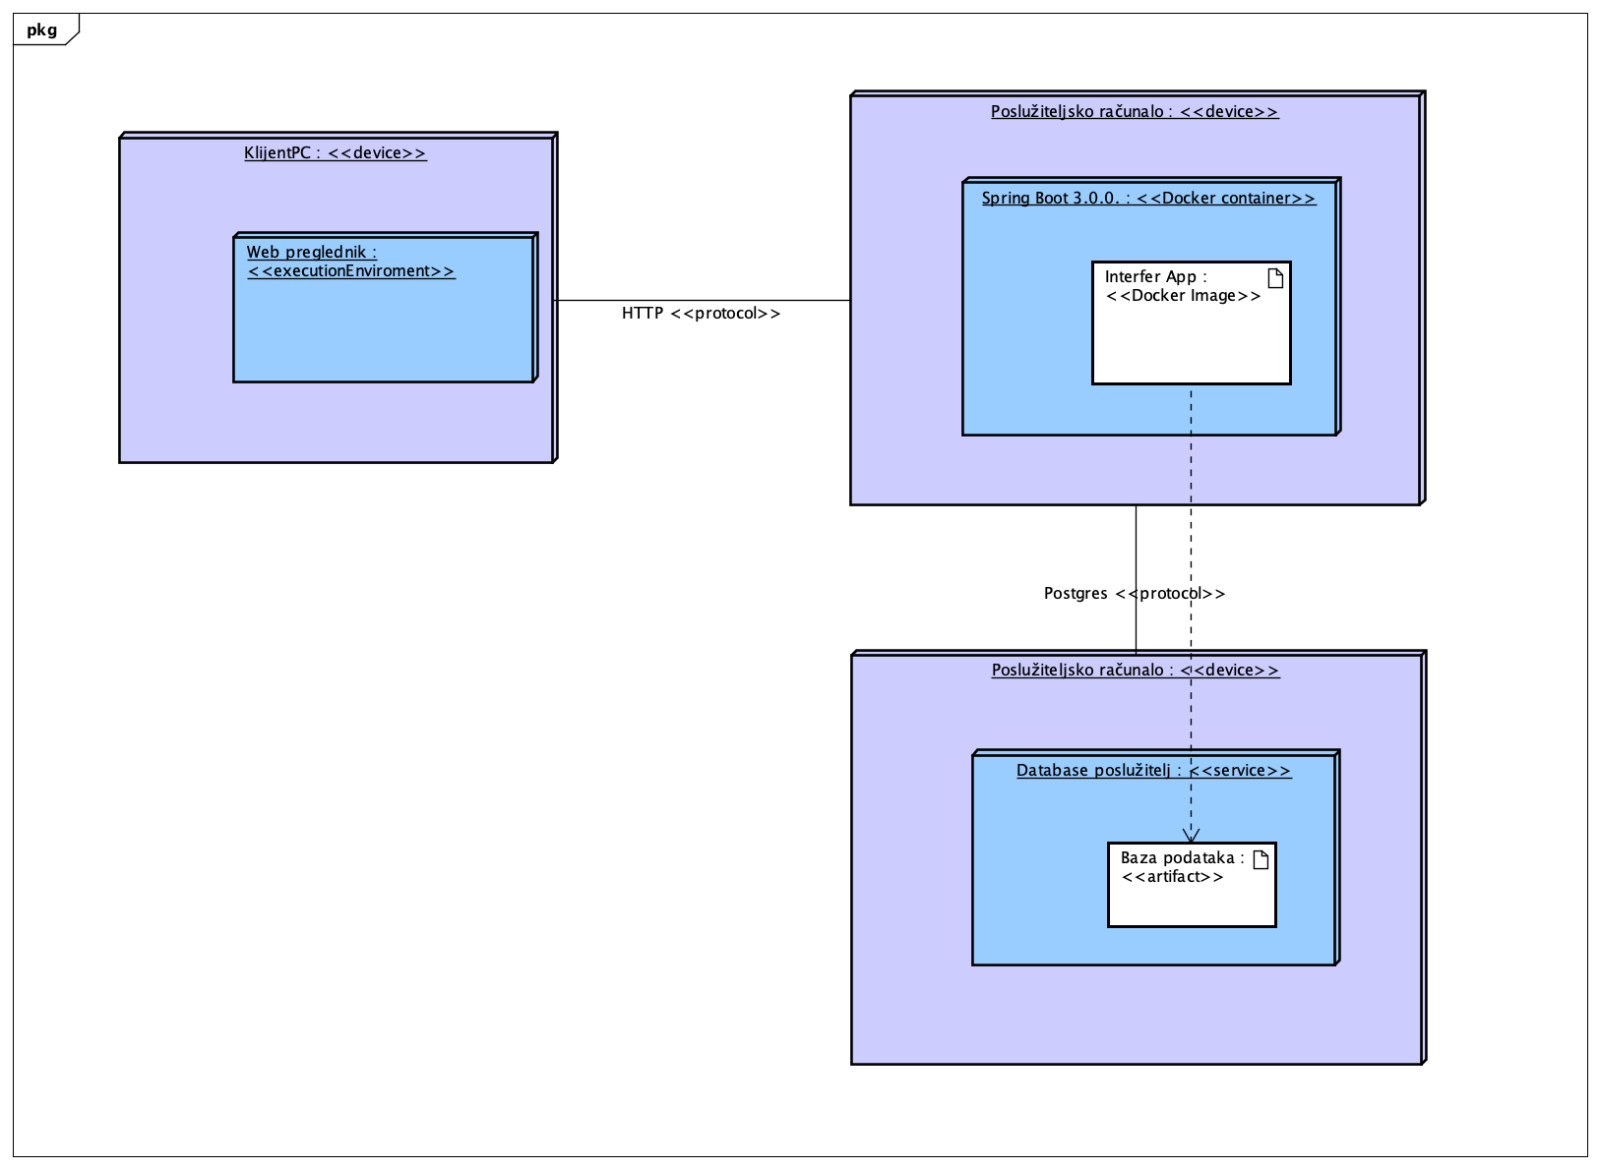
\includegraphics[scale=0.3]{slike/dijagram_razmjestaja.jpeg}
	\centering
	\caption{Dijagram Razmještaja}
	\label{fig:dijagram_razmjestaja}
\end{figure}

Opis UML dijagrama razmještaja za sustav komunikacije između dva 
poslužiteljska računala, jednog s Spring Boot 3.0.0. poslužiteljem i drugog s 
poslužiteljem baze podataka, pruža uvid u organizaciju elemenata sustava. Ovaj 
dijagram naglašava strukturu i komunikacijske veze u arhitekturi "klijent - 
poslužitelj".

Na prvom poslužiteljskom računalu smješten je Spring Boot 3.0.0. poslužitelj, 
čija je uloga centralna u obradi i upravljanju poslovnim logikama sustava. 
Ovaj poslužitelj komunicira s drugim poslužiteljem, gdje se nalazi baza 
podataka Postgres, čime se uspostavlja stabilna veza za pohranu i dohvaćanje 
podataka. Ova jasna podjela omogućuje učinkovito upravljanje podacima unutar 
sustava.

Klijenti, bilo da su korisnici, zaposlenici, vlasnici ili administratori, 
pristupaju sustavu putem web preglednika. U arhitekturi "klijent - poslužitelj
", komunikacija između računala korisnika i poslužitelja odvija se putem HTTP 
veze. Ova veza osigurava siguran prijenos podataka, omogućujući interakciju s 
web aplikacijom na intuitivan način. Kroz korištenje HTTP veze, pruža se 
skalabilnost i pristupačnost sustava, što je ključno za korisničko 
iskustvo.

Dijagram razmještaja također naglašava važnost organizacije komponenti sustava
, pružajući uvid u strukturu i međusobne veze poslužitelja, baze podataka i 
klijentskih računala. Ova organizacija ključna je za održavanje performansi i 
dostupnosti sustava, pridonoseći time ukupnoj stabilnosti i 
funkcionalnosti.

Sustav temeljen na ovakvoj arhitekturi omogućuje učinkovitu komunikaciju 
između svih elemenata, pridonošenje sigurnosti podataka putem HTTP veze, te 
osigurava optimalnu izvedbu sustava. Osim toga, organizacija elemenata na 
razmještajnom dijagramu omogućuje lako praćenje i upravljanje svim dijelovima 
sustava, čime se olakšava održavanje i daljnji razvoj.
			
			\eject 
		
		\section{Upute za puštanje u pogon}
		
U nastavku su navedeni koraci za puštanje u pogon web aplikacije koja uključuje
: PostgreSQL bazu podataka, Java Spring backend, i React.js frontend na javni 
poslužitelj Render. (https://render.com)

Render omogućuje besplatno posluživanje PostgreSQL baze podataka i web servisa 
koji će se koristiti u nastavku. Osim toga spajanjem na gitHub nudi mogućnost 
CI/CD modela posluživanja.

\subsection{Stvaranje baze na javnom poslužitelju}

Potrebno je otići na dashboard.render.com/new/database te popuniti formu. 
Potrebno je navesti jedinstveno ime instance PosrgreSQL-a, ime baze te ime 
korisnika kao npr:

\begin{figure}[H]
	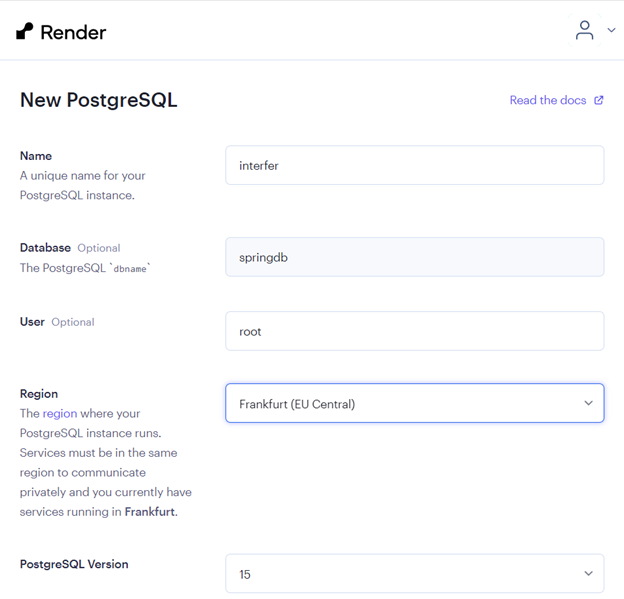
\includegraphics[scale=0.4]{slike/render_db.png}
	\centering
	\caption{Render - Nova PostgreSQL baza podataka}
	\label{fig:render_db1}
\end{figure}

Render će stvoriti bazu podataka a podacima ju popunjava sama aplikacija. 
Podatke za spajanje s bazom moguće je pronaći na dashboard-u.

\begin{figure}[H]
	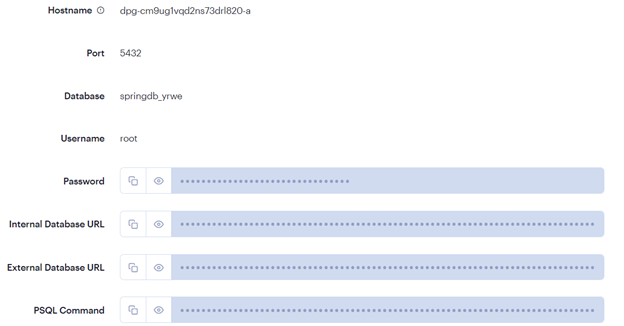
\includegraphics[scale=0.4]{slike/render_db1.png}
	\centering
	\caption{Render - Baza podataka}
	\label{fig:render_db2}
\end{figure}

\subsection{Konfiguriranje backenda}

Kako bi se spring aplikacija mogla spojiti na bazu potrebno je dodati 
dependency org.postgresql.postgresql u pom.xml, te zadati podatke za spajanje 
na bazu u IzvorniKod/backend/src/main/resources/aplication.properties. Za 
navedeni primjer potrebno je zadati:

spring.datasource.url=jdbc:postgresql://dpg-cm9ug1vqd2ns73drl820-a.frankfurt-postgres.render.com/springdb_yrwe

spring.datasource.username=root

spring.datasource.password=<zaporka>

spring.jpa.properties.hibernate.jdbc.lob.non_contextual_creation=true

spring.jpa.hibernate.ddl-auto=update

\subsection{Posluživanje backenda}

Potrebno je na Renderu napraviti instancu web servisa. Render za to nudi dvije 
mogućnosti:

\begin{figure}[H]
	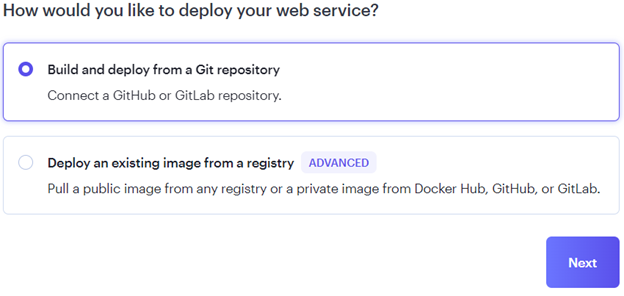
\includegraphics[scale=0.4]{slike/render_backend.png}
	\centering
	\caption{Render - Stvaranje web servisa}
	\label{fig:render_backend1}
\end{figure}

U ovim uputama opisat ćemo kako stvoriti servis iz git repozitorija (za to je 
potrebna prijava putem gitHub računa). U sljedećem koraku potrebno je odabrati 
repozitorij te postaviti konfiguracije:

\begin{figure}[H]
	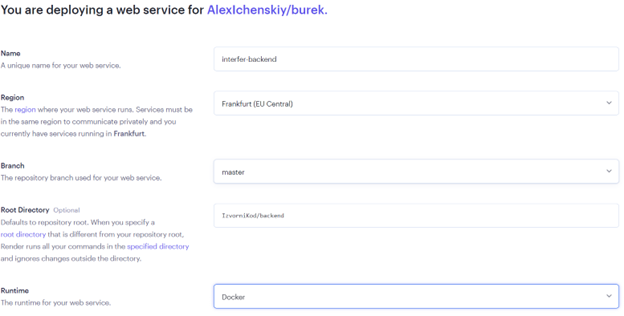
\includegraphics[scale=0.4]{slike/render_backend1.png}
	\centering
	\caption{Render - konfiguriranje web servisa}
	\label{fig:render_backend2}
\end{figure}

Poslužitelj gradi Docker sliku iz Dockerfile-a u navedenom direktoriju te ju 
poslužuje.

\subsection{Konfiguriranje frontenda}

Potrebno je u IzvorniKod/frontend/src/assets/constants.js zadati API_URL na 
kojemu je poslužen backend.

\subsection{Posluživanje frontenda}

Frontend se poslužuje na isti način kao backend, jedino je u postavkama 
umjesto IzvorniKod/backend potrebno za root directory zadati IzvorniKod/
frontend.

\eject 